\documentclass{article}
\usepackage[left=2cm,right=2cm,top=2cm,bottom=2cm]{geometry} 
\usepackage{graphicx} 
\usepackage[spanish]{babel}
%\usepackage[section]{placeins} 

%------------------------------ Constants ---------------------------------
\newcommand{\nombre}{Renato Flores - Manejo e implementacion de Archivos A-}
\newcommand{\carnet}{201709244}
\newcommand{\titulo}{Asistencia Conferencia Una Revolucion llamada Cubesat}
%----------------------- Custom commands ------------------------------
\author{\nombre , \carnet}
\title{\textbf{\Huge\titulo}}

\begin{document}
\maketitle

\begin{figure}[h]
        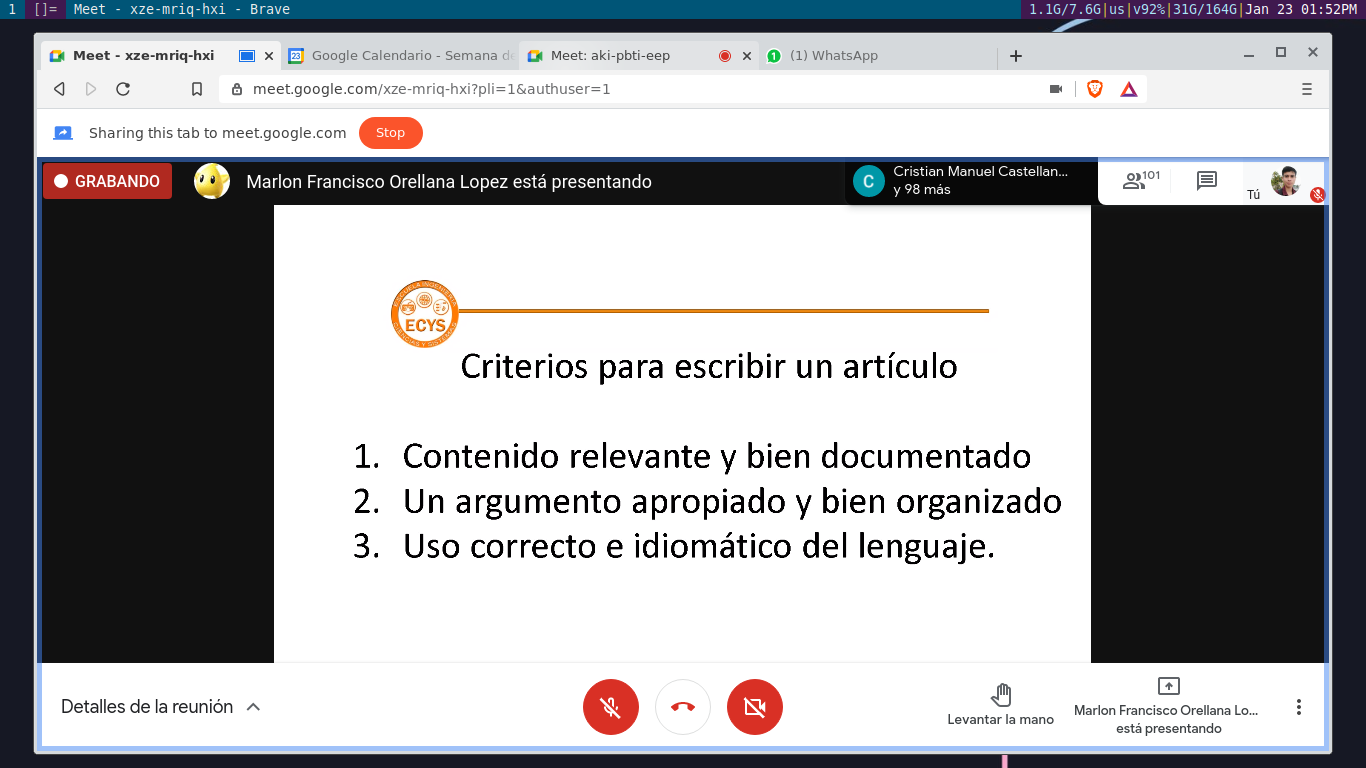
\includegraphics[width=\textwidth,keepaspectratio]{inicio.png}
		 \caption{Esperando confirmacion para poder entrar}
\end{figure}	
\pagebreak
\begin{figure}[h]
        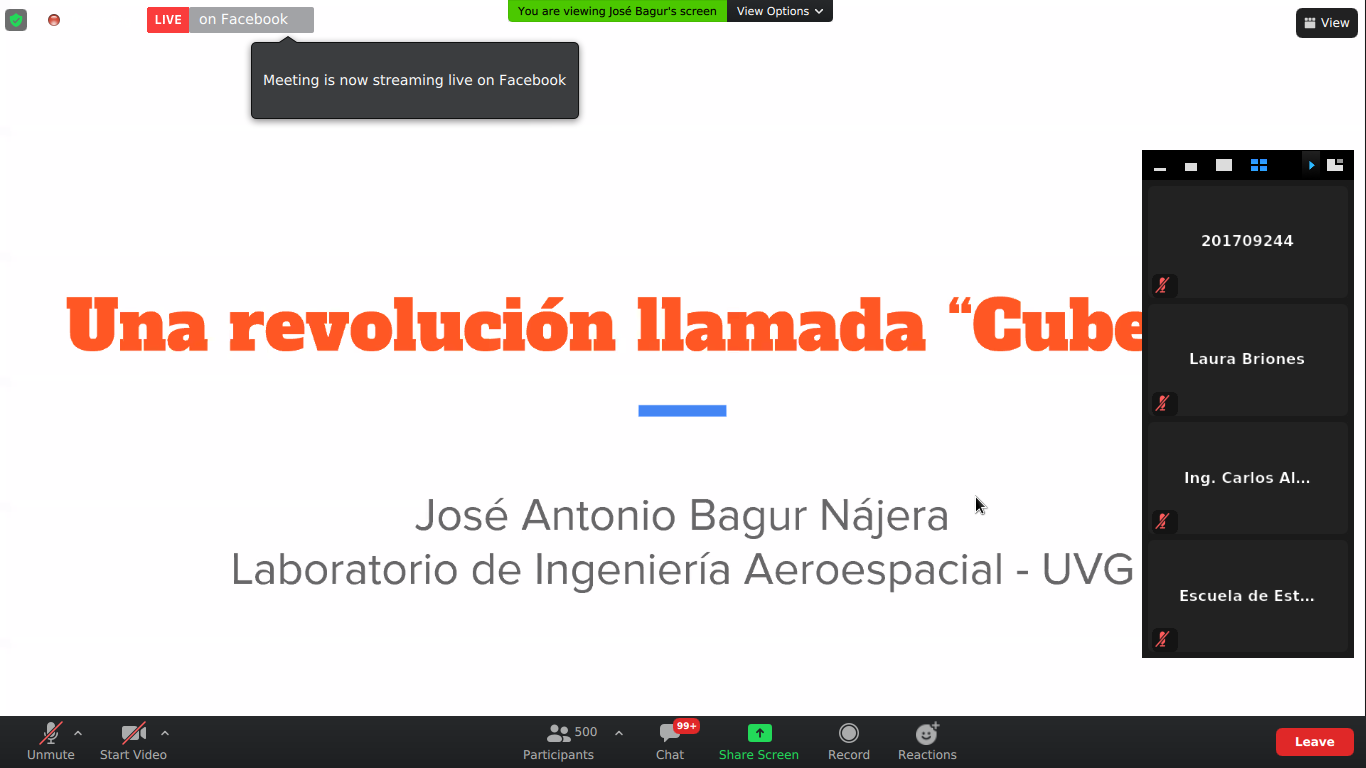
\includegraphics[width=\textwidth,keepaspectratio]{inicio-2.png}
		 \caption{En la reunion, pero esperando a que
		 de comienzo la conferencia}
\end{figure}
\pagebreak

\begin{figure}[h]
        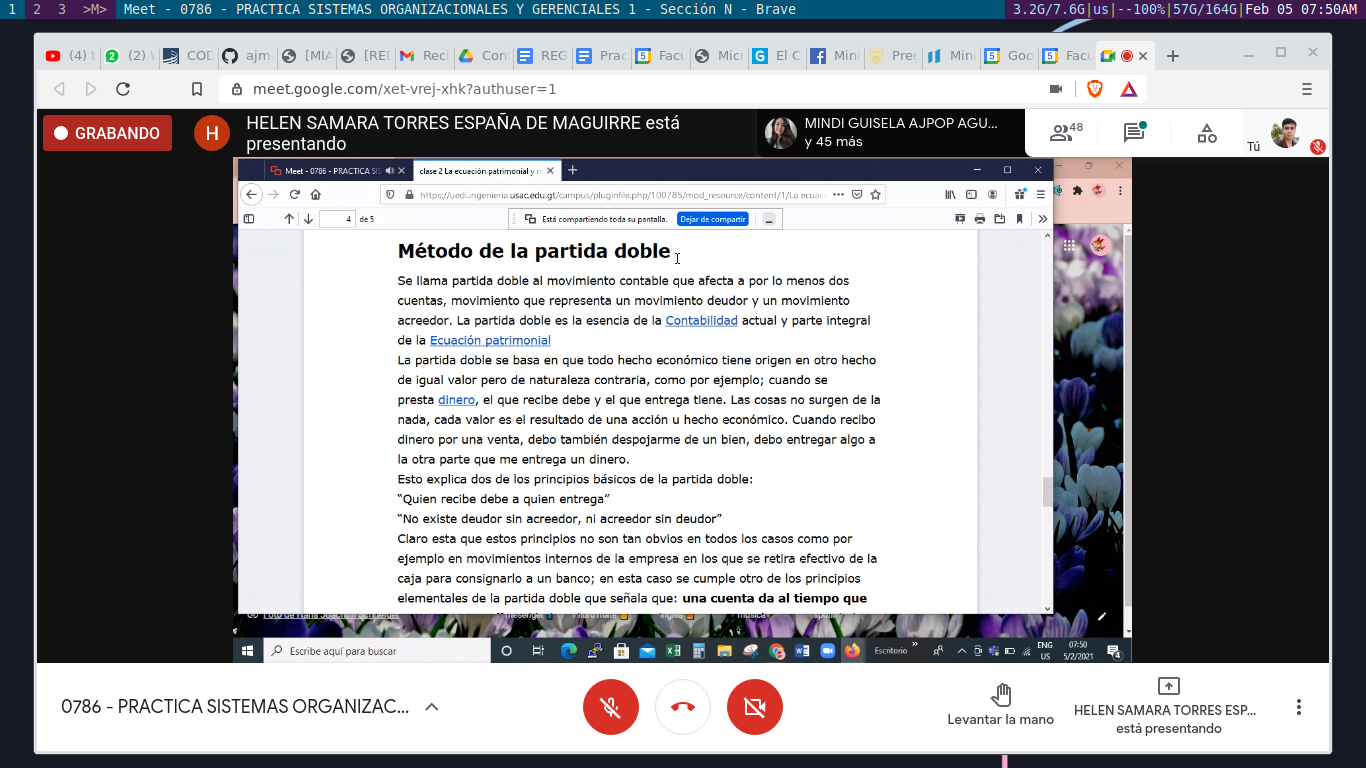
\includegraphics[width=\textwidth,keepaspectratio]{inicio-3.png}
		 \caption{Inicio de la conferencia}
\end{figure}

\begin{figure}[h]
        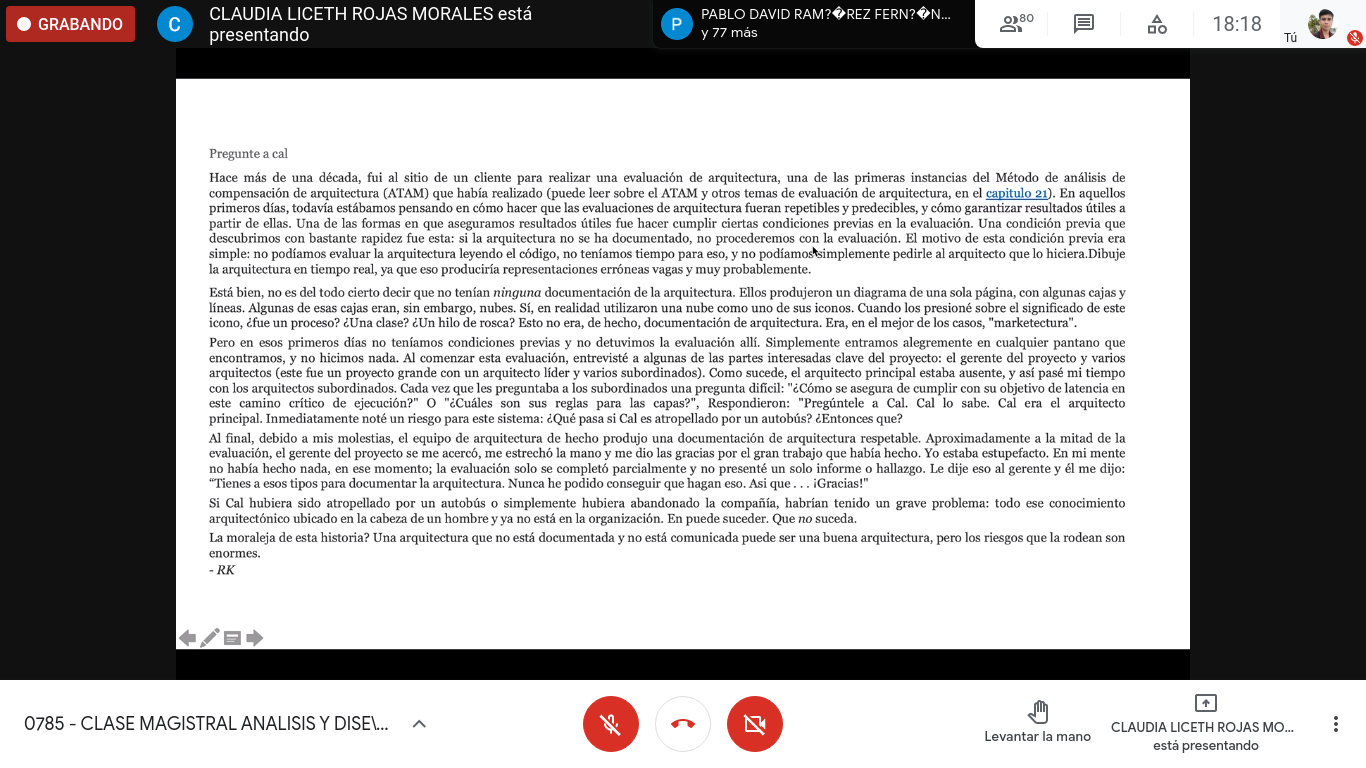
\includegraphics[width=\textwidth,keepaspectratio]{final.png}
		 \caption{Momentos finales de la reunion}
\end{figure}
\pagebreak

\begin{figure}[h]
        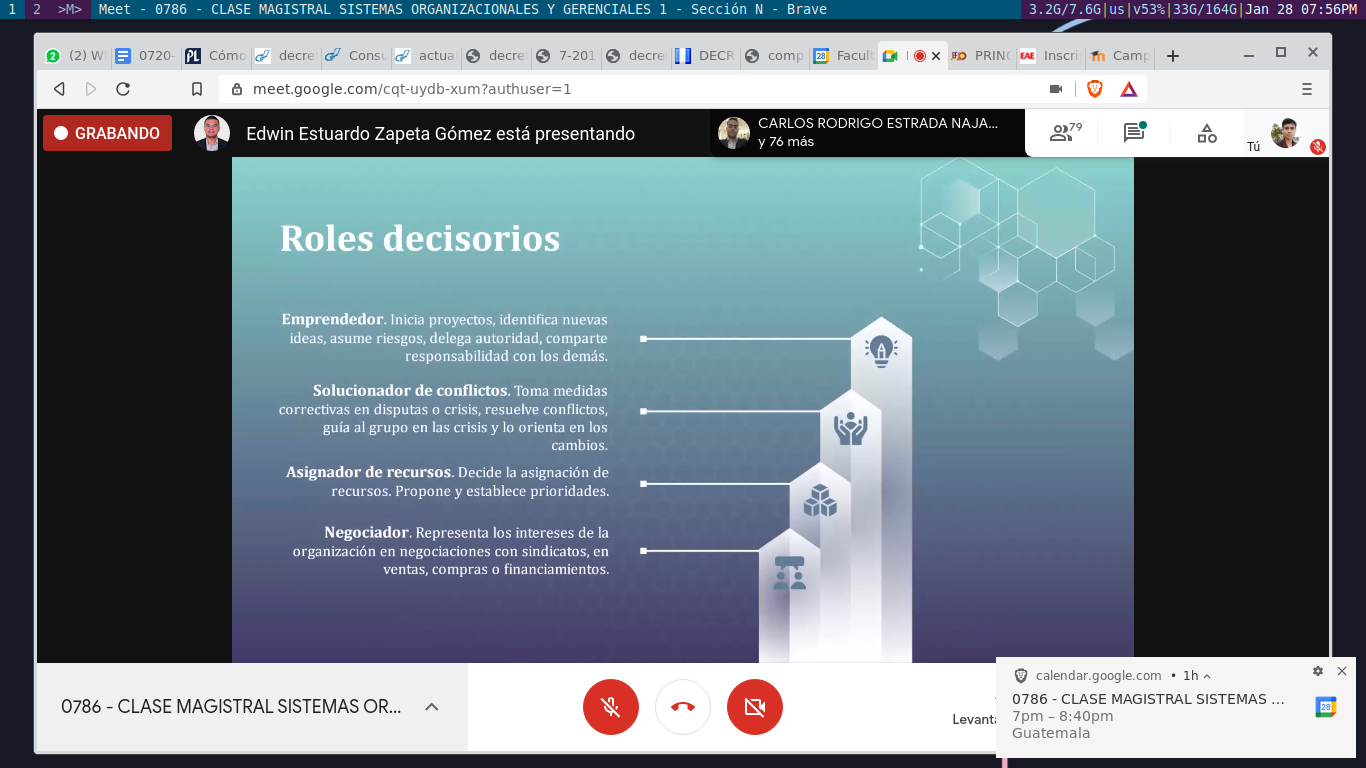
\includegraphics[width=\textwidth,keepaspectratio]{final-2.png}
		 \caption{Despedida de la conferencia}
\end{figure}
\end{document}
